\StartChapter{Differentialgleichungen (S.81,82,142)}

\SubsectionBar{Eigenschaften}
\textVorBox{Eine \ZSFkeyword{Differentialgleichung} enth\"alt Funktionen und deren Ableitungen.
Eine \ZSFkeyword{gew\"ohnliche Differentialgleichung (DGL)} h\"angt nur von einer Variablen (z.B. $x$) ab und ist von der Form:}
\begin{formulabox}
    $\displaystyle F(C,x,y'(x),y''(x),\ldots,y^{(n)}(x))=0$
\end{formulabox}
\textNachBox{wobei $C$ eine Konstante und $y$ eine Funktion in $x$ ist. Die h\"ochste Ableitung gibt die \ZSFkeyword{Ordnung der DGL} an.}

Die Menge der L\"osungen einer solchen Gleichung wird als die \ZSFkeyword{allgemeine L\"osung} der DGL bezeichnet. Sie bildet eine Schar von Funktionen mit einem \ZSFkeyword{Scharparameter} $C$.

Bei einer bekannten Bedingung $y(x_0)=y_0$, man spricht von einem \ZSFkeyword{Anfangswertproblem (AWP)}, kann der Scharparameter $C$ bestimmt werden. Die zugeh\"orige L\"osung der DGL wird als \ZSFkeyword{spezielle L\"osung} bezeichnet.

\SubsectionBar{Differentialgleichungen 1. Ordnung}
Sei $f(x,y)$ eine stetige und nach $y$ partiell stetig differenzierbare Funktion. Der \ZSFkeyword{Existenzsatz} besagt, dass f\"ur jeden Punkt $(x_0,y_0)$ genau eine Funktion $y(x)$ mit $y'=f(x,y)$ und $y(x_0)=y_0$ existiert. Graphisch bedeutet dies, dass die Graphen verschiedener Anfangswertprobleme entweder identisch sind oder sich nicht kreuzen.

\ZSFdanger{Achtung:} Ist $f(x,y)$ \textit{nicht} nach $y$ partiell stetig differenzierbar, k\"onnen zwei Funktionen $y(x)$ existieren, die $y'=f(x,y)$ erf\"ullen.
Eine DGL 1. Ordnung ist \ZSFkeyword{separierbar}, wenn sie in die folgende Form \"uberf\"uhrt werden kann:
\begin{formulabox}
    $\displaystyle y' = f(x,y) = \frac{g(x)}{h(y)}$
\end{formulabox}

Einige DGLs lassen sich nur durch Substitution separieren:
\begin{enumerate}
    \item W\"ahle eine Substitution $u(x,y)$ und stelle nach $y$ um
    \item Leite den umgestellten Term nach $x$ ab (kann zu $u'$ Term f\"uhren) und setze $y'$ mit dem urspr\"unglichen Term gleich
    \item Die entstandene DGL 1. Ordnung enth\"alt $u'$ und $u$, die mittels Integration nach $u(x)$ aufgel\"ost werden kann
    \item Nun den urspr\"unglichen Term $u(x,y)$ mit $u(x)$ gleichsetzen und dann nach $y$ aufl\"osen
\end{enumerate}

\SubsectionBar{Vektorfeld}
\textVorBox{In einem \ZSFkeyword{Richtungsfeld} (z.B. einem Vektorfeld $\vec v$) wird jedem Punkt $(x_0,y_0)$ eine Steigung $y'=f(x_0,y_0)$ zugewiesen:}
\begin{formulabox}
    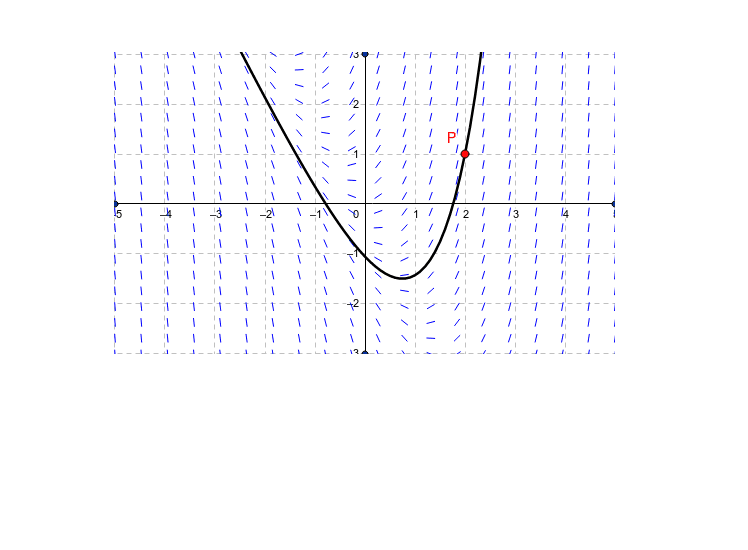
\includegraphics[width=\linewidth,keepaspectratio,trim=80 190 90 45,clip]{graphics/media/richtungsfeld_skizze.png}
\end{formulabox}

Fixiert man eine der Variablen (z.B. $x_0$) und variiert die andere (z.B. $y\in\R$), so erh\"alt man eine \ZSFkeyword{Kurvenschar}, eine Menge von Kurven. Solch eine \ZSFkeyword{einparametrige} Kurvenschar nennt man \ZSFkeyword{regul\"ar}, wenn sie keine Kreuzungspunkte aufweist.

\textVorBox{Die Steigung im Richtungsfeld berechnet sich mit:}
\begin{formulabox}
    $\displaystyle y'=\frac{v_2(x,y(x))}{v_1(x,y(x))}$
\end{formulabox}

\SubsectionBar{Lineare Differentialgleichungen}

\textVorBox{In einer \ZSFkeyword{linearen DGL 1. Ordnung (I)} d\"urfen $y$ und $y'$ nur als lineare Terme vorkommen:}
\begin{formulabox}
    $\displaystyle y'(x)=p(x)y(x)+q(x)$
\end{formulabox}
\textNachBox{Dabei ist $q(x)$ der \ZSFkeyword{inhomogene Teil}. Die zugeh\"orige \ZSFkeyword{homogene DGL (H)} lautet:
\[
    y'(x)=p(x)\,y(x).
\]
\ZSFdanger{Achtung:} Nicht erlaubt sind Terme wie $\cos(y')$, $y'y$ oder $y^2$.
Erlaubt sind hingegen lineare Terme wie $\sin(x)\cdot y$.}

Die allgemeine L\"osung von $I$ ist die Summe einer speziellen L\"osung (\ZSFkeyword{partikul\"are L\"osung} $y_p$) und der allgemeinen L\"osung $y_h$ von $H$.

\textVorBox{Ein erstes L\"osungsverfahren lautet:}
\begin{fulltablebox}{Z{1.0} | Z{1.0}}
    \ZSFrowColor
    \textbf{St\"orglied $q(x)$} & \textbf{Ansatz f\"ur $y_p$} \\ \hline
    Konstante & $C$ \\ \hline
    \ZSFrowColor
    Lineare Funktion & $C_1x + C_2$ \\ \hline
    Polynom mit Grad $n$ & $C_1\cdot x^n + C_2\cdot x^{n-1} + \dots$ \\ \hline
    \ZSFrowColor
    $C_1\cdot \sin(\omega x) + C_2\cdot \cos(\omega x)$ & $C_3\cdot \sin(\omega x) + C_4\cdot \cos(\omega x)$ \\ \hline
    $C_1\cdot e^{bx}$ & $C_2\cdot e^{bx}$ \\
\end{fulltablebox}

\begin{enumerate}
    \item Bestimme $y_h$ und w\"ahle ein $y_p$ mit passendem Ansatz
    \item Setze die Ableitungen von $y_p$ in $I$ ein
    \item Bestimme die Konstanten durch Koeffizientenvergleich
    \item Die allgemeine L\"osung ist $y(x)=y_p+y_h$
\end{enumerate}

\textVorBox{Ein zweites L\"osungsverfahren ist das nach Lagrange:}
\begin{enumerate}
    \item Bestimme $y_h$
    \item F\"uhre in $y_p=y(x)\cdot y_h(x)$ ein
    \item Leite $y_p$ ab und setze in $I$ ein
    \item Bestimme $y(x)$
    \item Die allgemeine L\"osung betr\"agt $y(x)=y_p+y_h$
\end{enumerate}

\SubsectionBar{Niveaulinien, Orth. trajektorien, Enveloppen}

\textVorBox{Sei $g(x,y)=C$ eine Schar von \ZSFkeyword{Niveaulinien}, so gilt:}
\begin{formulabox}
    $\displaystyle y'(x)=-\frac{g_x(x,y)}{g_y(x,y)}$
\end{formulabox}
\textNachBox{Eine solche DGL nennt man \ZSFkeyword{exakt} und kann umgeformt werden zu:
\[
    g_x(x,y)+y'(x)\,g_y(x,y)=0 \;\text{ mit }\; g_x=\psi_x.
\]
Die L\"osung ist die Schar von Niveaulinien $g(x,y)=C$.}

Die Niveaulinien von $g(x,y)$ stehen senkrecht auf den Feldlinien von $\nabla g(x,y)$, den sogenannten \ZSFkeyword{Orthogonaltrajektorien}.

\textVorBox{Sei $y'(x)=f(x,y)$ eine Kurvenschar, dann ist die Kurvenschar von Orthogonaltrajektorien gegeben durch:}
\begin{formulabox}
    $\displaystyle y_{\mathrm{or}}'(x)=-\frac{1}{y'(x)}$
\end{formulabox}

\textVorBox{Ein L\"osungsverfahren f\"ur Orthogonaltrajektorien lautet:}
\begin{enumerate}
    \item Schar nach $C$ umformen
    \item Urspr\"ungliche Schar nach $x$ ableiten und nach $y'$ aufl\"osen: $y'=f(x,y,C)$
    \item $C$ in abgeleiteter Schar durch Umformung aus (1) ersetzen
    \item $y'=f(x,y)$ in Formel f\"ur $y_{\mathrm{or}}'(x)$ einsetzen und die neue DGL l\"osen
\end{enumerate}

Die \ZSFkeyword{Enveloppe} einer Kurvenschar ist diejenige Kurve, die an jedem ihrer Punkte tangential zur Kurvenschar steht. Die zugeh\"orige L\"osung der DGL wird als \ZSFkeyword{singul\"are L\"osung} bezeichnet.

\textVorBox{Ein L\"osungsverfahren f\"ur Enveloppen lautet:}
\begin{enumerate}
    \item Sei die allgemeine L\"osung einer DGL $y=f(x,C)$ gegeben
    \item Nach $F(x,y,C)=0$ umstellen
    \item Mittels $F_C(x,y,C)=0$ den Scharparameter $C$ bestimmen
    \item Ausdruck f\"ur $C$ aus (3) in $F(x,y,C)=0$ einsetzen
\end{enumerate}

\SubsectionBar{Clairaut'sche Differentialgleichung}

\textVorBox{Clairaut'sche Differentialgleichungen sind von der Form:}
\begin{formulabox}
    $\displaystyle y = y'\cdot x + g(y')$
\end{formulabox}
\textNachBox{L\"osungen sind Geraden, eine singul\"are L\"osung und Kombinationen davon.}

\textVorBox{Ein L\"osungsverfahren f\"ur Clairaut'sche DGL lautet:}
\begin{enumerate}
    \item Setze $y'=C$ und erhalte die allgemeine L\"osung $y=Cx+g(C)$
    \item Leite nach $C$ ab und l\"ose nach $C$ auf
    \item Setze den Ausdruck aus (2) in die allgemeine L\"osung ein
\end{enumerate}

\SubsectionBar{Differentialgleichungen h\"oherer Ordnung}

\textVorBox{Eine \ZSFkeyword{Differentialgleichung h\"oherer Ordnung} ist von der Form:}
\begin{formulabox}
    $\displaystyle F\!\left(x,y,y'(x),y''(x),\ldots,y^{(n)}(x)\right)=0$
\end{formulabox}

Der Existenzsatz besagt, dass ein stetig differenzierbarer Anfangswert eine eindeutige L\"osung besitzt, durch jeden Punkt geht also genau eine Kurve ("regul\"ar").

\textNachBox{\ZSFdanger{Achtung:} Ist $f(x,y)$ nicht nach $y^{(1)}$ partiell stetig differenzierbar, hat die Funktion f\"ur ein AWP keine eindeutige L\"osung.}

\textVorBox{Eine \ZSFkeyword{lineare DGL h\"oherer Ordnung} ist von der Form:}
\begin{formulabox}
    $\displaystyle y^{(n)}(x)+p_{n-1}(x)y^{(n-1)}(x)+\dots+p_0(x)y(x)=q(x)$
\end{formulabox}
\textNachBox{Dabei sind $p_i(x)$ und $q(x)$ Funktionen.}

\begin{enumerate}
    \item Die lineare DGL ist \ZSFkeyword{homogen (H)}, wenn $q(x)=0$
    \item Linearkombinationen der L\"osungen von $H$ sind ebenfalls L\"osungen von $H$
    \item Die allgemeine L\"osung von $I$ ist eine Linearkombination aller linear unabh\"angigen L\"osungen von $H$
\end{enumerate}

\SubsectionBar{Homogene lineare DGL mit konst. Koeffizienten}

\textVorBox{Eine \ZSFkeyword{homogene lineare DGL mit konstanten Koeffizienten} ist von der Form:}
\begin{formulabox}
    $\displaystyle y^{(n)}(x)+a_{n-1}y^{(n-1)}(x)+\dots+a_0y(x)=0$
\end{formulabox}
\textNachBox{Dabei sind $a_i$ Konstanten.}

\textVorBox{Das \ZSFkeyword{charakteristische Polynom} einer solchen DGL lautet:}
\begin{formulabox}
    $\displaystyle P(\lambda)=\lambda^n+a_{n-1}\lambda^{n-1}+a_{n-2}\lambda^{n-2}+\dots+a_1\lambda+a_0$
\end{formulabox}
\textNachBox{Durch $P(\lambda)=0$ ergeben sich die Nullstellen.}

\begin{fulltablebox}{Z{0.8} | Y{1.2}}
    \ZSFrowColor \textbf{Nullstellen} & \textbf{L\"osungen} \\ \hline
    Einfach reell & $y(x)=e^{\lambda x}$ \\ \hline
    \ZSFrowColor
    Einfach komplex $(a=\alpha\pm ib)$ & \shortstack[l]{$e^{\alpha x}\cos(bx),$\\$e^{\alpha x}\sin(bx)$} \\ \hline
    k-fach reell & \shortstack[l]{$e^{\lambda x},\; x e^{\lambda x},\; \ldots,$\\$x^{k-1}e^{\lambda x}$} \\ \hline
    \ZSFrowColor
    k-fach komplex $(a=\alpha\pm ib)$ & \shortstack[l]{$e^{\alpha x}\cos(bx),$\\$e^{\alpha x}\sin(bx),$\\$\ldots,$\\$x^{k-1}e^{\alpha x}\sin(bx)$} \\
\end{fulltablebox}

Die allgemeine L\"osung $y$ der homogenen DGL ist eine Linearkombination der einzelnen L\"osungen $y_i$:
\begin{formulabox}
    $\displaystyle y=C_1y_1+C_2y_2+\dots+C_iy_i$
\end{formulabox}

\SubsectionBar{Euler'sche Differentialgleichung}

\textVorBox{Eine \ZSFkeyword{Euler'sche Differentialgleichung} ist von der Form:}
\begin{formulabox}
    $\displaystyle a_n y^{(n)}(x)+\frac{a_{n-1}}{x}y^{(n-1)}(x)+\dots+\frac{a_0}{x^n}y(x)=q(x)$
\end{formulabox}
\textNachBox{Dabei sind $a_i$ Konstanten.}

\textVorBox{Das \ZSFkeyword{charakteristische Polynom} einer solchen DGL lautet:}
\begin{formulabox}
    $\displaystyle P(\lambda)=a_n\lambda(\lambda-1)\cdots(\lambda-n+1)+a_{n-1}\lambda(\lambda-1)\cdots(\lambda-n+2)+\dots+a_2\lambda(\lambda-1)+a_1\lambda+a_0$
\end{formulabox}
\textNachBox{Durch $P(\lambda)=0$ ergeben sich die Nullstellen.}

\textVorBox{Folgendes gilt:}
\begin{fulltablebox}{Z{0.8} | Y{1.2}}
    \ZSFrowColor \textbf{Nullstellen} & \textbf{L\"osungen} \\ \hline
    Einfach reell & $y(x)=x^{\lambda}$ \\ \hline
    \ZSFrowColor
    Einfach komplex $(a=\alpha\pm ib)$ & \shortstack[l]{$x^{\alpha}\cos(b\ln(x)),$\\$x^{\alpha}\sin(b\ln(x))$} \\ \hline
    k-fach reell & \shortstack[l]{$x^{\lambda},\; \ln(x)\,x^{\lambda},\; \ldots,$\\$\ln(x)^{k-1}x^{\lambda}$} \\ \hline
    \ZSFrowColor
    k-fach komplex $(a=\alpha\pm ib)$ & \shortstack[l]{$x^{\alpha}\cos(b\ln(x)),$\\$x^{\alpha}\sin(b\ln(x)),$\\$\ldots,$\\$\ln(x)^{k-1}x^{\alpha}\sin\!\bigl(b\ln(x)\bigr)$} \\
\end{fulltablebox}

Die allgemeine L\"osung $y$ der homogenen Euler'schen DGL ist die Summe aus $y_h$ und $y_p$. Die homogene L\"osung ist eine Linearkombination der oben berechneten Terme $y_i$:
\begin{formulabox}
    $\displaystyle y_h=C_1y_1+C_2y_2+\dots+C_iy_i$
\end{formulabox}

\textVorBox{Ein Ansatz f\"ur die partikul\"are L\"osung einer DGL der obigen Form ist:}
\begin{formulabox}
    $\displaystyle y_p=Aq(x)+B$
\end{formulabox}
\textVorBox{F\"ur die alternative Schreibweise $a_n\cdot x^n\cdot y^{(n)}(x)+\dots+a_0\cdot y(x)=q(x)$ kann man auch den folgenden Ansatz probieren:}
\begin{formulabox}
    $\displaystyle y_p=Aq(x)+B$
\end{formulabox}

\textNachBox{$A$ und $B$ werden durch Einsetzen von $y_p$ in die DGL und einen anschliessenden Koeffizientenvergleich gefunden.}

\SubsectionBar{Taylorreihen f\"ur DGLs}
\textVorBox{Sei $y(x)$ eine Funktion mit Potenzreihe:}
\begin{formulabox}
    $\displaystyle y(x)=\sum_{n=0}^{\infty} c_nx^n$
\end{formulabox}
\textNachBox{So liefert ein Koeffizientenvergleich die L\"osung zugeh\"origer DGLs.}

\textVorBox{Sei die folgende DGL 2. Ordnung:}
\begin{formulabox}
    $\displaystyle y''+p_1(x)y'+p_0(x)y=q(x)$
\end{formulabox}
\textNachBox{Wenn $p_1$ und $p_0$ eine konvergierende Potenzreihenentwicklung um $x_0$ haben, dann gilt dies auch f\"ur $y(x)$.}
